\documentclass[12pt]{article}
\usepackage[inner=2.0cm,outer=2.0cm,top=2.5cm,bottom=2.5cm]{geometry}
\usepackage{float}
\usepackage{graphicx}
\usepackage{hyperref}
\setlength\voffset{-0.25in}
\setlength\textheight{675pt}

\usepackage{titling}
\setlength{\droptitle}{19em}
\title{CS 3651 - Prototyping Intelligent Devices\\ Mid-Project Review \\Wall-E}
\author{Names: Nithya Jayakumar, Tri Le}
\date{\today}


\begin{document}
\maketitle

\newpage
\begin{itemize}
    \item[1.] \textbf{A high-level design of the Wall-E Robot:}
    \begin{itemize}
        \item The electronic parts that are currently use
        \begin{itemize}
            \item[1)] Arduino Nano [x1]
            \begin{itemize}
                \item[+] Serving as the primary microcontroller, the Arduino Nano will execute the robot’s code, coordinating various actions and responses.
            \end{itemize}
            \item[2)] Buck Converter [x1]
            \begin{itemize}
                \item[+] Serving as voltage converter from the AA batteries to the Arduino and other electronic parts.
            \end{itemize}
            \item[3)] DC Geared Motors [x2]
            \begin{itemize}
                \item[+] These motors drive the wheels, allowing the robot to move forward, backward, and turn in response to objects detect by the Ultrasonic sensor.
            \end{itemize}
            \item[4)] Servos [x3]
            \begin{itemize}
                \item[+] Used to control the movement of the robot’s head rotation, and arms, servos add dynamic and expressive qualities to the robot’s appearance.
            \end{itemize}
            \item[5)] Ultrasonic Sensor [x1]
            \begin{itemize}
                \item[+] This sensor allow the robot to detect obstacles and avoidance it, allow it move safely.
            \end{itemize}
            \item[6)] Infrared Sensors (IR) [x2]
            \begin{itemize}
                \item[+] The IR sensors will placed near the robot eye, since it can't detect far object, this sensors purpose as something the user can interact with the robot, example hand movement in front of the robot, allow the robot to rotate it head and body to where the hand at.
            \end{itemize}
            \item[7)] Buzzer [x1]
            \begin{itemize}
                \item[+] This will make some sounds for the robot.
            \end{itemize}
            \item[9)] H-Bridge [x1]
            \begin{itemize}
                \item[+] This will responsible for controlling the DC motors that drive the robot’s movement, the H-Bridge facilitates precise control over speed and direction..
            \end{itemize}
            \item[10)] Red, Yellow and Green LEDs [x1]
            \begin{itemize}
                \item[+] These LEDs will serve as battery level check, since Wall-E have the battery level display, this is somewhat serve same purpose.
            \end{itemize}
            \item[11)] Blue and White LEDs [x1]
            \begin{itemize}
                \item[+] These LEDs will be the robot eyes, nornmal is blue, and when there is object detect, it will change to white.
            \end{itemize}
        \end{itemize}
        How they will be electrically connected, at a high level
        \begin{figure}[H]
            \centering
            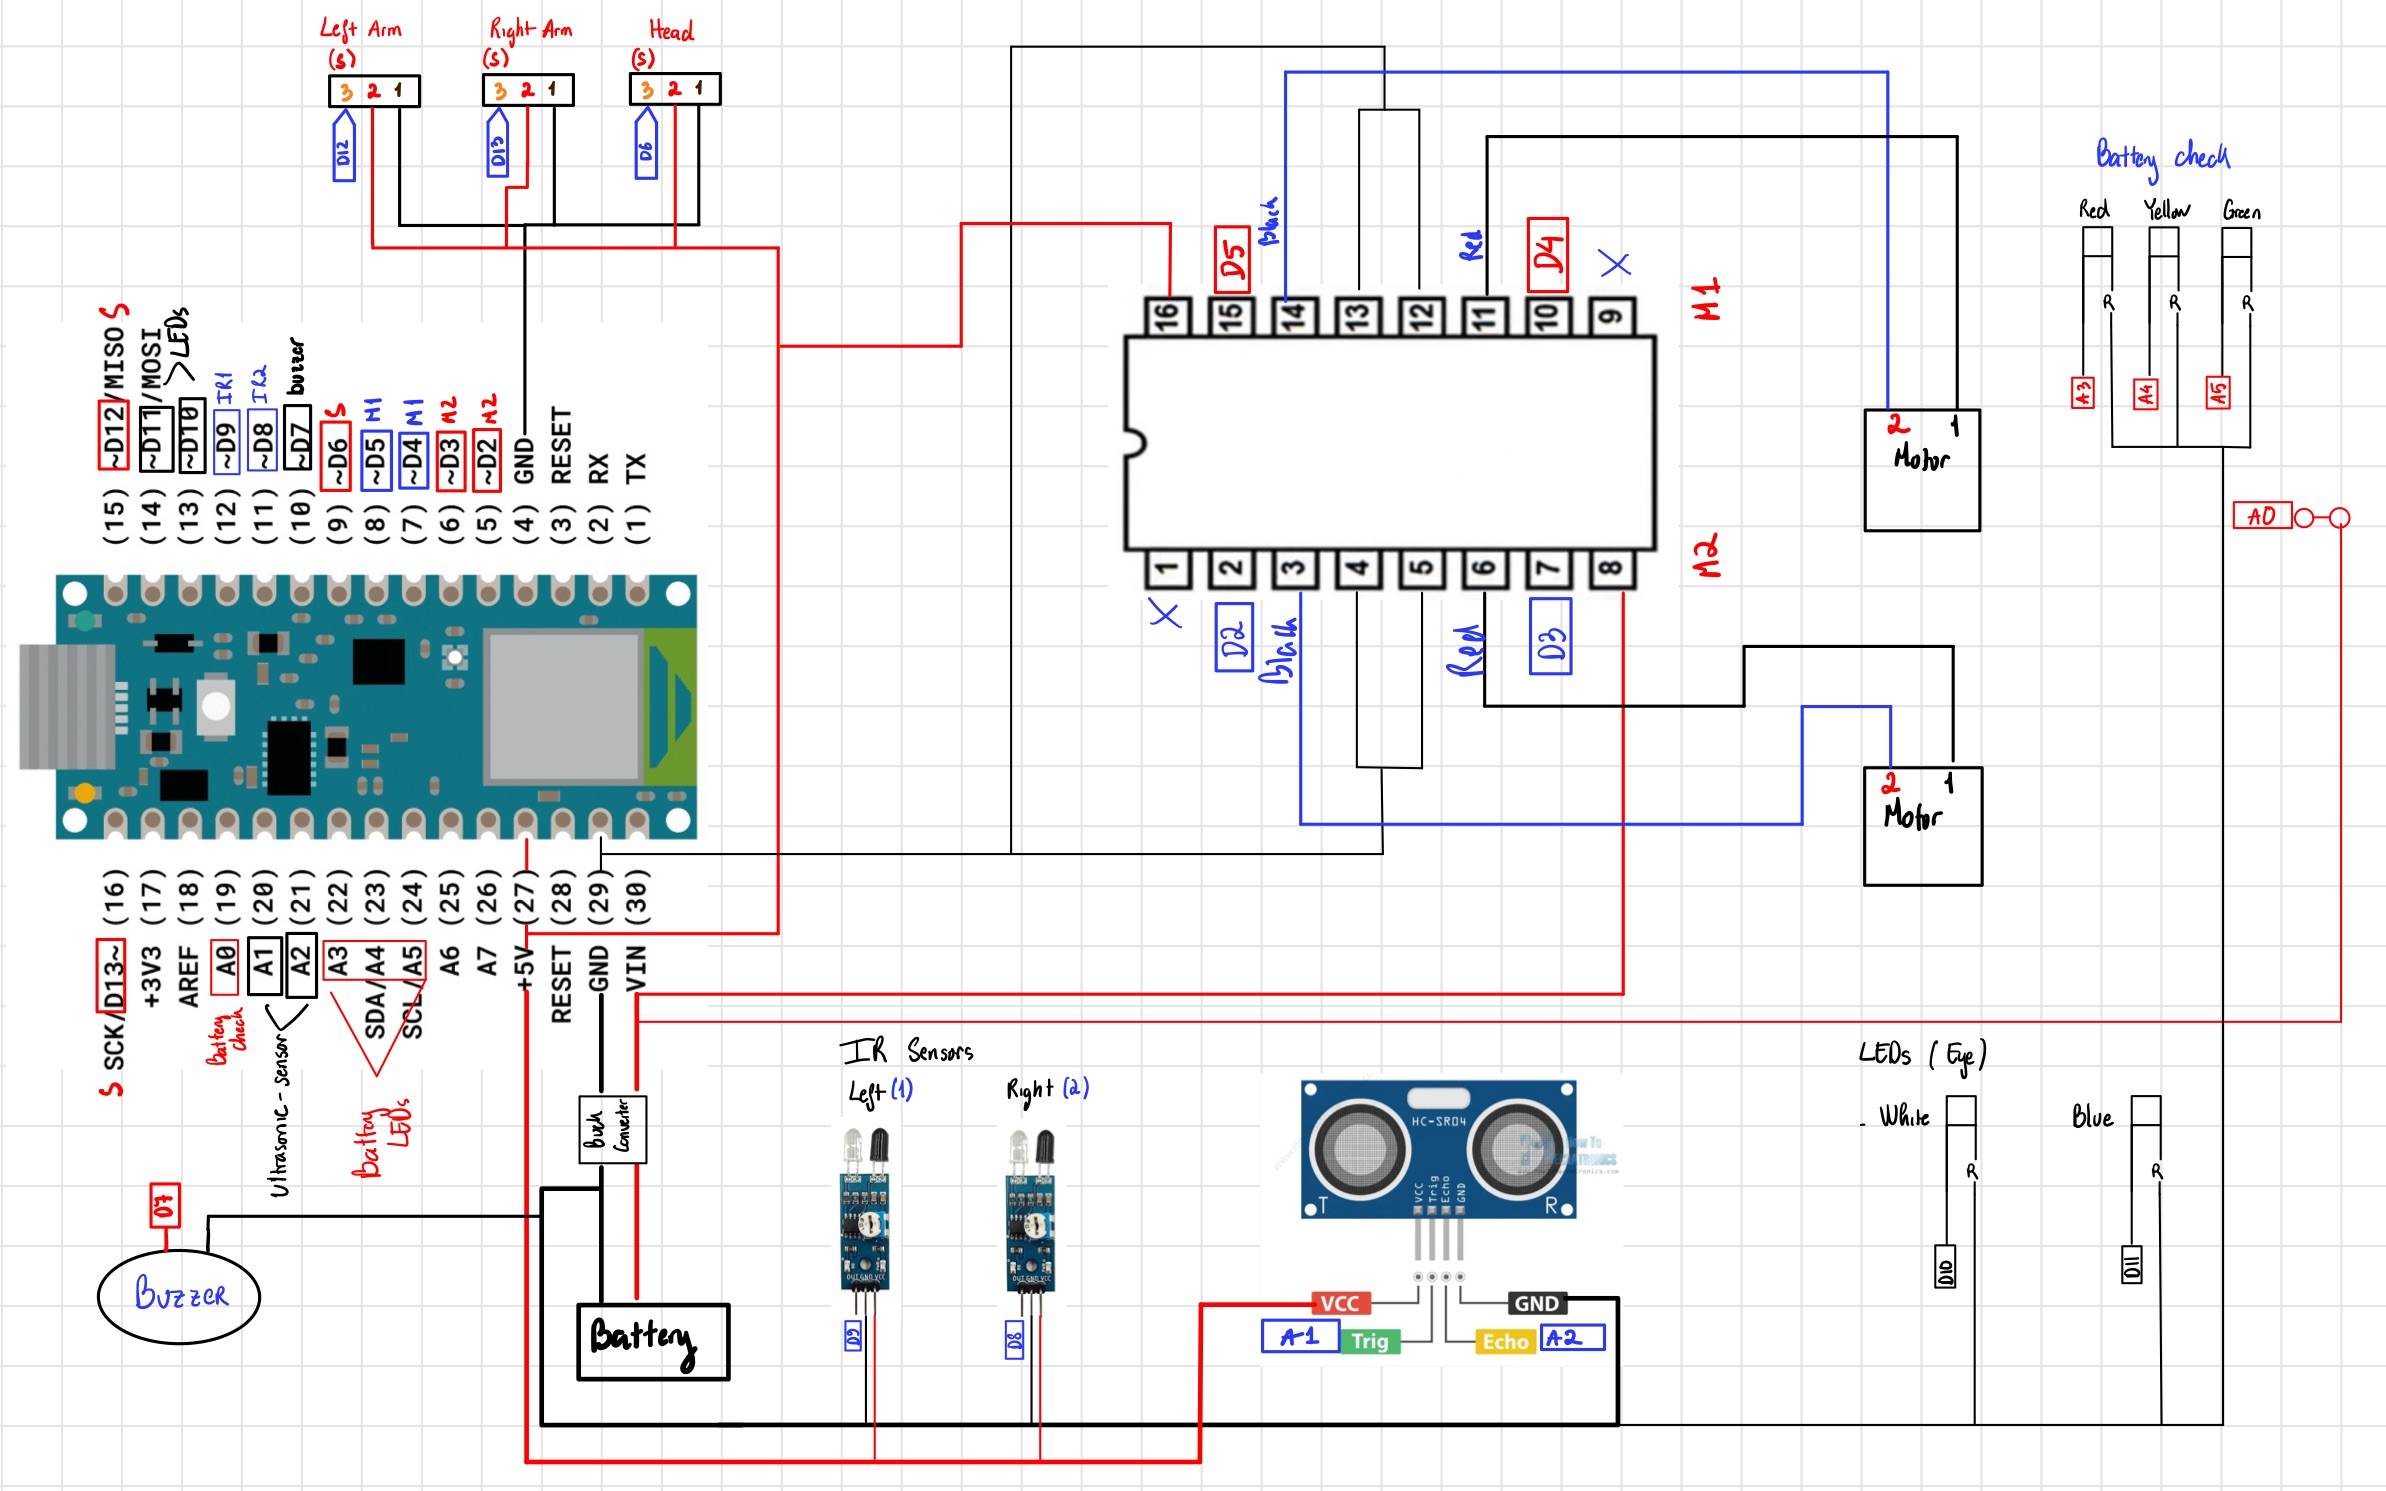
\includegraphics[width=500pt]{Project-1.jpg}
            \label{fig:enter-label}
        \end{figure}
        \item What software libraries you are using
        \begin{itemize}
            \item[+] Servo.h and NewPing.h
        \end{itemize}
        \item What mechanical parts you plan to make
        \begin{itemize}
            \item[+] Battery Compartment - a compartment will be designed to securely hold the AA batteries, ensuring they are protected and easily accessible for replacement when needed.
            \item[+] Modified Wall-E Eye - the eye of the Wall-E Robot will be modified to accommodate LEDs and IR sensors. This modification will enhance the robot's functionality and interaction capabilities.
            \item[+] Body Modification for Sensors and LEDs -  part of the robot's body will be modified to house the ultrasonic sensor and LEDs for battery indication. 
        \end{itemize}
    \end{itemize}
    \item[2.] \textbf{Team progress:}
    \begin{itemize}
        \item Any goals already achieved from your proposal: Yes, several milestones outlined in the proposal have been successfully completed:
        \begin{itemize}
            \item[+] Constructed the robot's brain, including wiring, soldering parts, and assembling components.
            \item[+] Partially 3D printed the robot's exterior, including body parts, wheels, and tracks. Other parts are currently in the printing process.
            \item[+] Implemented basic movement capabilities: the robot can move forward and detect obstacles using the ultrasonic sensor, turning left or right when obstacles are detected.
            \item[+] Implemented functionality for the IR sensor and head servo: when a hand is detected close to the eye, the head and body move in that direction. Further improvements are in progress.
            \item[+] The team is currently revising electronic parts and finalizing wire soldering.
        \end{itemize}
        \item Physical components of the project that you have:
        \begin{itemize}
            \item[a)] Have in-hand:
            \begin{itemize}
                \item[+] Servos, ultrasonic sensor, IR sensors, buck converter, Arduino Nano, buzzer, DC geared motors, H-bridge, LEDs.
            \end{itemize}
            \item[b)] Have tested:
            \begin{itemize}
                \item[+] IR sensor and servo functionality.
                \item[+] LEDs for battery level indication.
            \end{itemize}
            \item[c)] Have integrated
            \begin{itemize}
                \item[+] Arduino Nano.
                \item[+] H-bridge with DC geared motors for movement control.
                \item[+] Servos for head and arm movement.
                \item[+] Ultrasonic sensor for obstacle detection.
                \item[+] Buck converter and AA batteries for power supply.
            \end{itemize}
        \end{itemize}
    \end{itemize}
    \item[3.] \textbf{Difficulties encountered:}
    \begin{itemize}
        \item Ways we can work around parts of your original design that aren't going to come together in time
        \begin{itemize}
            \item[-] In the team proposal, we said we would implement mapping for the robot. However, after discussions with the TA and Scott, we believe it's best to leverage the use of sensors instead. This approach would be more feasible and effective. Additionally, while our proposal mentioned the use of Bluetooth, we still aim to incorporate something similar for the final deliverable if time allows.
        \end{itemize}
        \item Is there anything you wish was covered in a skill demo?
        \begin{itemize}
            \item[-] Perhaps demonstrating how to desolder components could be valuable. Additionally, covering how to properly utilize batteries with Arduino would be beneficial.
            \item[-] Additionally, it would have been helpful to have a skill demo that deals with assembling mechanical parts in order to understand and internalize concepts such as space for wiring and parts as well as connections
        \end{itemize}
    \end{itemize}
\end{itemize}
\end{document}